\section{Arquitectura SNN base para detección de anomalías en series temporales}
\label{sec:arquitectura-snn-base}

Una vez comprendidos los fundamentos de las SNNs, en esta sección se describe la arquitectura SNN base, específicamente diseñada para la detección de anomalías en series temporales, que constituye el punto de partida para la solución propuesta en el \hyperref[chap:especificacion]{Capítulo 3}.

% \subsubsection{Motivación y principio de funcionamiento}

% La hipótesis fundamental de este enfoque es que una SNN entrenada con datos normales mediante STDP exhibirá patrones de disparo característicos al procesar dichos datos. Cuando la red se enfrenta a datos anómalos o con comportamientos diferentes a los aprendidos, los patrones de disparo cambiarán significativamente. Específicamente, se espera que la frecuencia de generación de impulsos sea distinta al procesar datos normales frente a datos anómalos.

% Esta aproximación aprovecha las propiedades inherentes de las SNNs: su capacidad de aprendizaje no supervisado mediante STDP y su sensibilidad a los patrones temporales de la información de entrada.

\subsection{Arquitectura bicapa}

El modelo SNN base consta de dos capas principales, denominadas A y B:

\paragraph{Capa A (entrada).} Esta capa actúa como interfaz entre los datos de entrada y la red neuronal. Su función es transformar los valores continuos de la serie temporal en impulsos discretos. El número de neuronas en esta capa es 39.

\paragraph{Capa B (procesamiento).} Compuesta por 100 neuronas LIF completamente conectadas a la capa A. Esta capa presenta dos características distintivas:

\begin{itemize}
    \item Conexiones propagación hacia adelante desde la capa A: cada neurona de la capa B recibe entradas ponderadas desde todas las neuronas de la capa A.
    \item Conexiones recurrentes dentro de la propia capa B: las neuronas están interconectadas entre sí, permitiendo que los impulsos generados en esta capa influyan en el estado de las demás neuronas del mismo nivel. Estas conexiones recurrentes son fundamentales para capturar dependencias temporales en los datos.
\end{itemize}

\begin{figure}[!htb]
    \centering
    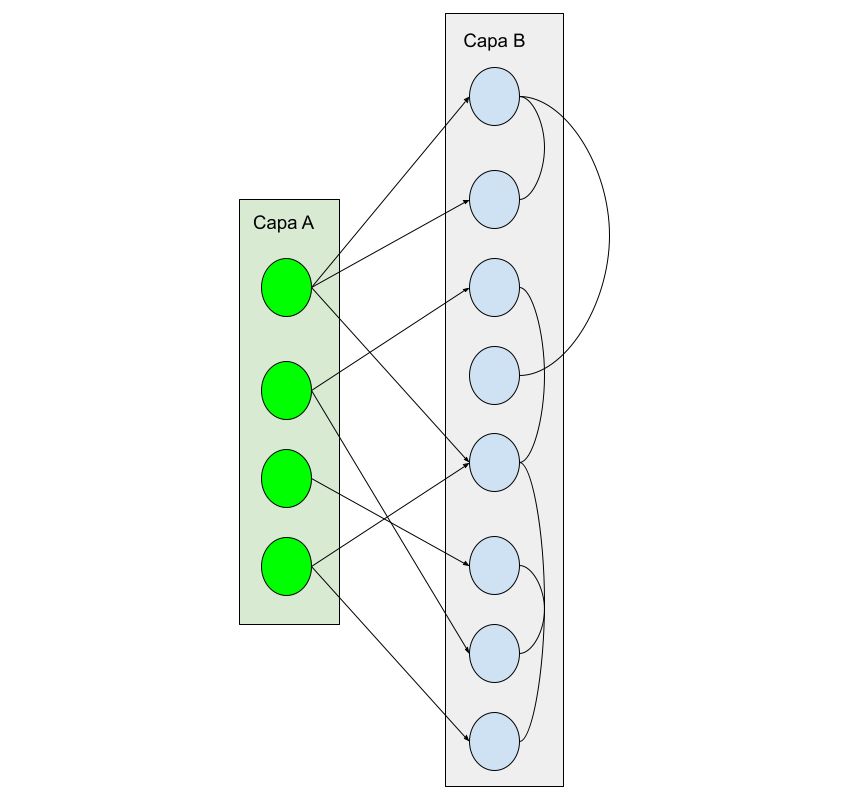
\includegraphics[width=0.8\textwidth]{Imagenes/Diagrama de capas de SNN Base.png}
    \caption{Diagrama de la arquitectura bicapa de la SNN base. Inspirado en \cite{vazquez_vacuum_2024}.}
    \label{fig:arquitectura-bicapa-snn}
\end{figure}

\subsection{Codificación por cuantiles}

Para convertir valores continuos de series temporales en impulsos discretos, se emplea una estrategia de codificación basada en cuantiles estadísticos. Este método divide el rango de valores observados en el conjunto de entrenamiento en intervalos disjuntos, donde cada intervalo corresponde a una neurona de la capa A.

El proceso funciona de la siguiente manera:

\begin{enumerate}
    \item Durante la fase de preparación, se calculan los cuantiles de la distribución de valores en los datos de entrenamiento. Por ejemplo, si se eligen $n$ cuantiles, se obtienen $n-1$ neuronas en la capa A.
    \item Cada valor de la serie temporal se asigna al intervalo que le corresponde según su magnitud.
    \item La neurona asociada a dicho intervalo genera un impulso en el instante temporal actual.
    \item Este impulso se propaga a la capa B a través de las conexiones sinápticas.
\end{enumerate}

Esta codificación presenta ventajas importantes: es determinista, computacionalmente eficiente y adapta automáticamente la representación a la distribución estadística de los datos específicos del problema. Además, valores fuera del rango original pueden ser manejados mediante intervalos adicionales en los extremos.

\subsection{Aprendizaje mediante STDP modificado}

El entrenamiento de la red se realiza mediante una variante de STDP diseñada específicamente para la tarea de detección de anomalías. A diferencia del STDP clásico, donde se refuerzan conexiones que conducen a disparos postsinápticos inmediatos, aquí se emplea una estrategia de penalización bidireccional.

El mecanismo funciona de la siguiente forma:

\begin{itemize}
    \item Se penalizan las conexiones hacia neuronas que hayan emitido impulsos recientemente (impulsos presinápticos).
    \item También se penalizan las conexiones hacia neuronas que disparen inmediatamente después del impulso actual (impulsos postsinápticos).
\end{itemize}

Esta doble penalización tiene como objetivo inhibir la generación de impulsos cuando la red procesa datos normales, es decir, datos similares a los observados durante el entrenamiento. La intuición es que, si la red ha aprendido correctamente los patrones normales, debería generar pocos impulsos al encontrarlos nuevamente. En cambio, ante datos anómalos, las conexiones ajustadas no serán efectivas para suprimir la actividad, resultando en un mayor número de impulsos.

Los parámetros de aprendizaje nu1 y nu2 controlan la magnitud de los ajustes sinápticos en las conexiones A→B y B→B respectivamente. Estos valores son típicamente negativos para implementar la penalización descrita.

\subsection{Criterio de detección de anomalías}

Una vez entrenada la red, la detección de anomalías se basa en la frecuencia de impulsos generados por la capa B durante la inferencia. El procedimiento es el siguiente:

\begin{enumerate}
    \item Durante el procesamiento de nuevos datos, se monitoriza la actividad de disparo de las neuronas en la capa B.
    \item Se calcula una métrica agregada de la actividad neuronal, típicamente la suma de impulsos en una ventana temporal deslizante.
    \item Esta señal de actividad se suaviza mediante técnicas como media móvil para reducir fluctuaciones instantáneas.
    \item Se compara la actividad suavizada con un umbral estadístico predeterminado.
    \item Cuando la actividad supera el umbral, se genera una alerta de anomalía.
\end{enumerate}

El umbral puede establecerse mediante análisis estadístico de la actividad observada durante el procesamiento de datos de validación normales, por ejemplo, utilizando la media más dos desviaciones estándar.

\subsection{Limitaciones de la arquitectura base}

Aunque esta arquitectura demuestra la viabilidad de aplicar SNNs a la detección de anomalías, presenta varias limitaciones que motivan el desarrollo de mejoras:

\begin{itemize}
    \item Ausencia de extracción de características jerárquicas: la conectividad completamente conectada (fully-connected) no captura eficientemente patrones locales o estructuras temporales específicas, que son fundamentales para detectar anomalías sutiles en series temporales complejas.
    
    \item Sensibilidad a hiperparámetros: los parámetros nu1, nu2, el umbral de disparo y la constante de decaimiento deben ajustarse manualmente o mediante búsqueda exhaustiva, sin un mecanismo de optimización automatizada.
    
    \item Rendimiento limitado en presencia de ruido: en conjuntos de datos con alta variabilidad o ruido temporal, la red puede generar falsos positivos al interpretar variaciones normales como comportamientos anómalos.
    
    \item Escalabilidad computacional: aunque las SNNs son intrínsecamente eficientes, la ausencia de capas especializadas para reducción de dimensionalidad puede limitar su aplicación a series temporales de gran longitud o alta frecuencia de muestreo.
    
    \item Criterio de alerta simple: la decisión de anomalía se basa únicamente en estadísticas agregadas de impulsos en la capa B, sin aprovechar potencialmente múltiples representaciones o rutas de procesamiento paralelo.
\end{itemize}

Estas limitaciones serán abordadas en el \hyperref[chap:especificacion]{Capítulo 3} mediante la introducción de una arquitectura híbrida que combina la eficiencia de las SNNs con capacidades de procesamiento convolucional, optimización automatizada de hiperparámetros y estrategias de decisión más sofisticadas.

